\documentclass[12pt,a4paper,]{article}
\usepackage{lmodern}
\usepackage{amssymb,amsmath}
\usepackage{ifxetex,ifluatex}
\usepackage{fixltx2e} % provides \textsubscript
\ifnum 0\ifxetex 1\fi\ifluatex 1\fi=0 % if pdftex
  \usepackage[T1]{fontenc}
  \usepackage[utf8]{inputenc}
\else % if luatex or xelatex
  \ifxetex
    \usepackage{mathspec}
  \else
    \usepackage{fontspec}
  \fi
  \defaultfontfeatures{Mapping=tex-text}
    \setmainfont[]{Tinos}
\fi
% use upquote if available, for straight quotes in verbatim environments
\IfFileExists{upquote.sty}{\usepackage{upquote}}{}
% use microtype if available
\IfFileExists{microtype.sty}{%
\usepackage{microtype}
\UseMicrotypeSet[protrusion]{basicmath} % disable protrusion for tt fonts
}{}
\usepackage[unicode=true]{hyperref}
\hypersetup{
            pdfborder={0 0 0},
            breaklinks=true}
%\urlstyle{same}  % don't use monospace font for urls
\usepackage{natbib}
\bibliographystyle{unified}
\setlength{\emergencystretch}{3em}  % prevent overfull lines
\providecommand{\tightlist}{%
  \setlength{\itemsep}{0pt}\setlength{\parskip}{0pt}}
\setcounter{secnumdepth}{5}
% Redefines (sub)paragraphs to behave more like sections
\ifx\paragraph\undefined\else
\let\oldparagraph\paragraph
\renewcommand{\paragraph}[1]{\oldparagraph{#1}\mbox{}}
\fi
\ifx\subparagraph\undefined\else
\let\oldsubparagraph\subparagraph
\renewcommand{\subparagraph}[1]{\oldsubparagraph{#1}\mbox{}}
\fi

% set default figure placement to htbp
%\makeatletter
%\def\fps@figure{htbp}
%\makeatother

\usepackage{booktabs}
\usepackage{longtable}
\usepackage{array}
\usepackage{multirow}
\usepackage{wrapfig}
\usepackage{float}
\usepackage{colortbl}
\usepackage{pdflscape}
\usepackage{tabu}
\usepackage{threeparttable}
\usepackage{threeparttablex}
\usepackage[normalem]{ulem}
\usepackage{makecell}
\usepackage{xcolor}

\let\tnote\relax
\usepackage{cleveref}
\usepackage{ctable}
\usepackage{enumerate}
\usepackage{lineno}
\linenumbers

\date{}

\usepackage[absolute]{textpos}

\begin{document}
\begin{textblock}{3}(0.2,0.2)
  \textcolor{lightgray}{v1.1.9000 (2019/10/16)}
\end{textblock}

\large

TITLE: Temporal (in)stability in English monosyllabic and disyllabic
words: Insights on the effect of voicing on vowel duration

\vspace{1cm}

AUTHOR: Stefano Coretta

\vspace{1cm}

AFFILIATION: Linguistics and English Language, University of Manchester,
Oxford Road, Manchester, M13 9PL, United Kingdom

\vspace{1cm}

EMAIL ADDRESS:
\href{mailto:stefano.coretta@manchester.ac.uk}{\nolinkurl{stefano.coretta@manchester.ac.uk}}

\normalsize

\pagebreak

\begin{abstract}
English is one in the wide range of languages in which the duration of vowels is modulated by the voicing of the following consonant: Vowels are shorter when followed by voiceless stops, and longer when followed by voiced stops.
The so-called voicing effect has been attributed to a variety of mechanisms.
Temporal compensation between the duration of the vowel and the following stop closure is one of these mechanisms.
Based on acoustic data from Italian and Polish disyllabic words, the compensatory mechanism has been proposed to be a consequence of the temporal stability of the interval between the consonant releases flanking the vowel.
The timing of the VC boundary within this interval determines the respective durations of the vowel and the stop closure.
In this paper, it is shown that the duration of the release-to-release interval is not affected by the voicing of the second consonant in English disyllabic words, but that it is in monosyllabic words.
It is argued that the stability of the interval can be derived from the isochronous phasing of the vocalic gestures in the VCV sequence of disyllabic words.
The absence of the temporal anchor of a second vowel in monosyllabic words, on the other hand, allows the vocalic and the consonant gesture durations to be modified independently.
Other aspects of production and perception behind the voicing effect can coexist with a temporal compensation mechanism and cannot be excluded.
\end{abstract}

\textbf{Keywords}: voicing effect, vowel duration, compensatory
adjustment, English

\hypertarget{introduction}{%
\section{Introduction}\label{introduction}}

\label{s:intro}

A well-known cross-linguistic tendency is that vowels have shorter
durations when followed by voiceless stops and longer durations when
followed by voiced stops. This so-called `voicing effect' has been long
documented in a wide range of languages across different linguistic
families \citep{maddieson1976, begus2017}. Several hypotheses have been
proposed as to the origin of this phenomenon, from articulatory
mechanisms to perceptual biases; however, no one particular account has
gained universal support.

One such hypothesis, the compensatory temporal adjustment account,
states that the voicing effect involves a compensatory mechanism between
vowel and consonant closure duration. Vowels are shorter when followed
by voiceless stops because the latter have longer closure durations,
and, vice versa, vowels are longer before voiced stops because the
latter have shorter closure durations. However, the compensatory account
fails to clearly identify a speech interval within which compensation is
implemented. Both the syllable \citep{lindblom1967, farnetani1986} and
the word \citep{slis1969a, slis1969b, lehiste1970a, lehiste1970b} have
been proposed as such intervals, but these have been subsequently
criticised on empirical and logical grounds
\citep{chen1970, jacewicz2009, maddieson1976, coretta2019k}.

In an exploratory study of acoustic durations in Italian and Polish
trochaic CV́CV words, \citet{coretta2019k} finds that the duration of the
interval between the the release of C1 and the release of C2 (the
release-to-release interval) is not affected by the voicing status of
the second consonant. The duration of the release-to-release interval in
words where the second consonant is voiceless (like /pata/) is not
significantly different from that in words where the second consonant is
voiced (for example,
/pada/).\footnote{Note that the release-to-release interval is not equivalent to the VC interval, since the latter does not include the VOT from the consonant preceding the vowel. See \citet{coretta2019k} for further details.}
The temporal stability of the release-to-release interval is compatible
with a compensatory temporal adjustment account of the voicing effect
\citep{lindblom1967, slis1969a, slis1969b, lehiste1970a, lehiste1970b},
and it offers a resolution to the drawbacks of previous versions of the
account.

Given the temporal stability of the release-to-release interval, the
timing of the acoustic vowel/consonant (VC) boundary (corresponding to
the acoustic vowel offset and the acoustic consonant closure onset)
within that interval determines the respective durations of vowel and
consonant closure. Since the VC boundary in voiceless stops is timed
earlier within the release-to-release relative to voiced stops, the
vowel is shorter and closures is longer when the post-vocalic stop is
voiceless than when it is voiced. This interpretation agrees with known
differences of closure durations in voiceless vs.~voiced stops
\citep{lisker1957, van-summers1987, davis1989, de-jong1991}, namely that
voiceless closures are longer than voiced ones. Thus, a possible
diachronic pathway to the voicing effect is one in which vowel and
closure duration differences emerge from changes in the timing of the VC
boundary within the release-to-release interval.

Note that the release-to-release interval in itself does not have a
special status in the account put forward here. The proposed account of
compensatory temporal adjustment can be understood in relation to the
\textit{acoustic} duration of vowels, hence the scope of compensation
can (but need not) be defined in terms of acoustic intervals. As
reviewed above, the interval found to be temporally stable across
voicing contexts in disyllabic words in Italian and Polish is the
release-to-release interval \citep{coretta2019k}. However, it is
desirable to derive the isochrony of this acoustic interval from
properties of articulatory coordination. A tentative account of the
underlying gestural coordination from which the release-to-release
isochrony can be derived is offered here.

\hypertarget{a-gestural-account-of-the-voicing-effect}{%
\subsection{A gestural account of the voicing
effect}\label{a-gestural-account-of-the-voicing-effect}}

\label{s:gest}

According to \citet{ohman1966, ohman1967}, the speech stream is composed
by a series of continuous vocalic gestures interrupted by gestures of
oral constriction (consonants). \citet{fowler1983} further proposes that
the vocalic gestures of a VCV sequence are characterised by a cyclic
pattern of production, so that the temporal distance between the two
vowels is constant, independent of the nature of the intervening
consonant. While the temporal distance of the V-to-V interval is
modulated by the number of intervening consonants
\citep{zmarich2011, zeroual2015}, the distance can still be expected to
be stable within the context of disyllabic words with a single
intervocalic consonant that alternates in voicing.

The task-dynamic model \citep{saltzman2008} of Articulatory Phonology
\citep{ohala1986a, browman1988, browman1992}, based on the coupled
oscillators model \citep{odell2008}, states that any two gestures can be
implemented according to two modes. Either they are initiated in
synchrony or they are implemented sequentially. These modes of gestural
phasing (in-phase and anti-phase) can account for a variety of patterns
of articulatory timing. Onset consonants are generally produced in-phase
with the following vowel, meaning that the vocalic and consonantal
gestures are initiated together. This same mechanism also gives rise to
the so-called C-centre effects observed with onsets, by which the
acoustic duration of a vowel depends on the number of onset consonants
\citep{browman1988, marin2010, hermes2013, marin2014}. On the other
hand, coda consonants tend to be produced anti-phase relative to the
preceding vowel and to each other, meaning that they are articulated in
sequence. The duration of vowels has been found to be insensitive to the
number of coda consonants following them \citep{marin2010, marin2014}

Further evidence for a vowel-based rhythmic gestural implementation
comes from work by \citet{farnetani1986} and \citet{celata2014}. These
studies investigate the relation between vowel duration and syllable
structure in Italian. In the first study, it was found that vowels
followed by a singleton stop (for example in /la.da/) are longer than
vowels followed by a tautosyllabic cluster (/la.dra/). This pattern can
easily be derived from a scenario in which the distance between the
vowels is the same in the two contexts (/la.da/ and /la.dra/), and the
onset consonants follow a C-centre alignment. The onset of the first
consonant in the /dr/ cluster is shifted towards the vowel, making the
latter shorter. \citet{celata2014} also show that the duration of the
consonant/consonant cluster is negatively correlated with the duration
of the preceding vowel (although the magnitude of the correlation is low
to moderate).

Under the gestural account proposed in this paper, the combined action
of the isochrony of the vowel-to-vowel interval and the in-phase
alignment of the onset consonant is responsible for the isochrony of the
release-to-release interval in CVCV words. The first consonant and vowel
are produced in-phase with each other, and these are sequentially
followed by the second consonant and vowel, again produced in-phase with
each other. Then, the differential duration found in the voicing effect
would be a consequence of the different velocity of the closing gesture
in voiceless vs.~voiced consonants.

\citet{van-summers1987} shows that the closing gesture of voiceless
stops has greater velocity than that of voiced stops. Assuming that the
closing gesture of both voiceless and voiced stops is initiated in
synchrony with that of the following vowel (as per the in-phase
alignment), full oral closure is achieved earlier in voiceless stops
relative to its timing in voiced stops. The result is, everything else
being equal, a shorter vowel and a longer (full) closure in voiceless
stops, and a longer vowel and a shorter closure in voiced stops.
\citet{warren2006} offer some evidence from lip data, where the lip
closing gestures (together with the jaw gesture) accounts for about 80\%
of the vowel duration difference.

A similar chain of reasoning applies to the context of coda consonants.
If coda consonants are produced anti-phase with the preceding vowel and
the closing gesture of the consonant starts at a specific time after the
production of the vowel independent of consonant voicing, then the
greater velocity of the closing gesture in voiceless stops would result
in a shorter vowel and a longer closure relative to voiced stops.
However, the articulatory data in \citet{de-jong1991} suggests that the
timing of the onset of the stop closing gesture differs depending on
voicing in English monosyllabic words. \Cref{s:gen-disc} will discuss a
possible solution based on perceptual mechanisms that could reconcile
the articulatory predictions put forward here and the empirical data.

\hypertarget{the-voicing-effect-in-english}{%
\subsection{The voicing effect in
English}\label{the-voicing-effect-in-english}}

\label{s:ve-eng}

English is one of the most investigated languages in relation to the
voicing effect
\citep{meyer1904, heffner1937, house1953, belasco1953, peterson1960, halle1967, chen1970, klatt1973, lisker1974, laeufer1992, fowler1992, hussein1994, lampp2004, warren2005, durvasula2012, ko2018}.
English is also the language in which the voicing effect reportedly has
the greatest magnitude relative to that of other languages. This special
status of English is traditionally attributed to the phonologisation of
the voicing effect in this language \citep{sharf1964, de-jong2004}.
Vowel duration and the vowel-to-consonant duration ratio are considered
to be among the most stable cues to consonantal voicing
\citep{peterson1960, raphael1972, port1982}. \citet{kluender1988}
proposed that the difference in vowel duration before voiceless
vs.~voiced stops could have been enhanced and exploited to cue the
voicing contrast. This could explain the greater effect of English
compared for example to the effect in Italian, in which voicing is most
robustly cued by vocal fold vibration during closure \citep{pape2014}.

As it is the case, previous studies on English have reported a
difference in vowel duration before voiceless vs.~voiced stops which
ranges between 20 and 150 ms, while the values for the effect in Italian
are lower, between 15 and 25 ms
\citep{caldognetto1979, farnetani1986, esposito2002, coretta2019k}. A
Bayesian meta-analysis of the voicing effect based on estimates obtained
from 15 studies suggests that the effect of voicing in English
monosyllabic words ranges between 55 and 95 ms at 95\% probability, with
a meta-analytical mean of 75 ms (see Supplement A). On the other hand,
the meta-analytical estimate of the voicing effect for disyllabic words
is lower, at about 25 ms (around 50 ms less than in monosyllabic words).
This estimate is closer to the effect sizes reported for Italian. Note,
however, that the Italian values refer to the effect as observed in
disyllabic words.

Nevertheless, it is possible that the alleged differences in magnitude
between English and other languages are a product of the different
contexts under examination \citep{laeufer1992}. \citet{ko2018}, in a
more recent investigation of the voicing effect in English monosyllabic
words, finds a substantially lower difference in vowel duration (35 ms).
The Bayesian meta-analysis (Supplement A) further suggests a potential
for publication bias towards bigger effects, which means that the
meta-analytical estimate (75 ms) could be an overestimation. Finally,
the surveyed studies have a very low number of participants (mean = 3.4,
SD = 2.5), which can lead to so-called Type M errors (estimate magnitude
errors) and overestimation of the effect
\citep{kirby2018, roettger2019}. In sum, it is generally assumed that
the voicing-driven differences in vowel duration are greater in English
than in other languages, although the empirical foundation of this
conception is not entirely straightforward. Although not the focus of
this study, arguments based on differences in effect size will become
relevant when discussing the results.

\hypertarget{research-hypotheses}{%
\subsection{Research hypotheses}\label{research-hypotheses}}

\label{s:hypo}

One of the aims of this study is to test whether the same temporal
stability observed for the release-to-release interval in Italian and
Polish disyllabic words can also be observed in English. English makes a
good object of enquiry since much work on the voicing effect has been
done on this language, and the phonological structure of the language
allows us to directly compare onset and coda stops in disyllabic and
monosyllabic words respectively. While the temporal stability of the
release-to-release interval is expected in English disyllabic words,
monosyllabic words are predicted not to show such stability. As
discussed above, an essential component of the release-to-release
temporal stability in disyllabic words is the presence of a direct
relation between the two vowels in these type of words. Since
monosyllabic words don't have a second vowel, there is no direct
vowel-to-vowel relation to derive the release-to-release stability from.

Furthermore, \citet{jacewicz2009} report that, in American English,
monosyllabic words are longer when the second consonant is voiced. Based
on this finding, it is expected that the release-to-release duration
should be longer when C2 is voiced. \citet{jacewicz2009} attribute the
difference in monosyllabic word duration to the difference in vowel
duration before voiceless vs.~voiced stops. Thus, we can expect the
magnitude of the difference in release-to-release duration in
monosyllabic words to be close to the difference in vowel duration. This
hypothesis also fits with the reported greater effect of voicing on
vowel duration in monosyllabic than disyllabic words (with the caveats
discussed in \Cref{s:ve-eng}).

The data in \citet{coretta2019k} suggests that the intrinsic duration of
vowels and consonants can contribute to the duration of the
release-to-release interval. In particular, release-to-release intervals
containing a high vowel have shorter durations than those with a low
vowel. This is not surprising, given the well-known tendency of high
vowels to be shorter than low vowels
\citep{hertrich1997, esposito2002, mortensen2013, toivonen2015, kawahara2017}.
As for the consonantal place of articulation, the release-to-release is
shorter in Italian and Polish when the second consonant is velar
compared to when it is coronal. This could be a consequence of the fact
that the closure of velar stops is shorter than that of other stops. For
example, \citeauthor{sharf1962}'s (\citeyear{sharf1962}) data on closure
duration in English suggests that the closure of labial stops (60-90 ms)
is about 10 ms longer than that of velar stops (55-75 ms). It can be
expected that release-to-release intervals with a velar stop in English
will be about 10 ms shorter than intervals with a labial stop.

Another set of objectives concerns the effect of voicing on vowel and
closure durations. A conceptual replication of previous studies' effect
sizes is sought, with special attention to differences between
monosyllabic and disyllabic words. Only a few studies directly compare
the effect on vowel durations in different syllabic positions (for
example, \citet{sharf1962} and \citet{klatt1973}). The reported effects
are in the range of 50-55 ms in word-final (closed-syllable) position
and 20-25 in word-medial (open-syllable) position. The Bayesian
meta-analysis of the voicing effect indicates a mean difference of 50 ms
(75 ms in word-final position vs.~25 ms word-medially). As for the
duration of stop closure, the data in \citet{sharf1962} and
\citet{luce1985} indicates that voiced closures are 10-13 ms shorter
than voiceless closures.

While directly investigating the statistical relationship between vowel
and closure durations might seem more appropriate for assessing whether
a compensation exists between the two, this was not done for three
reasons. First, as discussed by \citet{ohala1976} and \citet{begus2017},
interpreting the correlations between two temporal intervals that share
a boundary is problematic, unless one uses two independent sources for
the measurements of vowel and closure durations, such as multiple
annotators \citep{begus2017} or articulatory data from different
articulators \citep{de-jong1991}. Neither of these options were
available for this study due to time and resources constraints. Second,
as discussed in \citet{coretta2019k}, less is known about the interplay
between segment durations, speech rate, and the vowel/closure relation,
making interpretation of data on correlation difficult in most cases. A
third reason for not correlating vowel and closure durations is that the
main focus of this study was to assess word-level gestural phasing via
acoustic measures. Future work will have to be carried out in which the
vowel/closure correlation is investigated using robust and unambiguous
methods.

To summarise, the following research questions and respective hypotheses
can be formulated:

\begin{enumerate}
\def\labelenumi{\arabic{enumi}.}
\tightlist
\item
  Is the duration of the interval between two consecutive stop releases
  (the release-to-release interval) in monosyllabic and disyllabic words
  affected by the voicing of C2 in English?
\end{enumerate}

\begin{itemize}
\tightlist
\item
  H1a: The duration of the release-to-release interval is not affected
  by C2 voicing in disyllabic words.
\item
  H1b: The release-to-release interval is longer in monosyllabic words
  with a voiced C2 than in monosyllabic words with a voiceless C2.
\end{itemize}

\begin{enumerate}
\def\labelenumi{\arabic{enumi}.}
\setcounter{enumi}{1}
\tightlist
\item
  Is the duration of the release-to-release interval affected by (a) the
  number of syllables of the word, (b) the quality of V1, and (c) the
  place of C2?
\end{enumerate}

\begin{itemize}
\tightlist
\item
  H2a: The release-to-release interval is longer in monosyllabic than in
  disyllabic words.
\item
  H2b: The duration of the release-to-release interval decreases
  according to the hierarchy /ɑː/, /ɜː/, /iː/.
\item
  H2c: The release-to-release interval is longer when C2 is labial.
\end{itemize}

\begin{enumerate}
\def\labelenumi{\arabic{enumi}.}
\setcounter{enumi}{2}
\tightlist
\item
  What is the estimated difference in the effect of voicing on vowel and
  stop closure duration between monosyllabic and disyllabic words?
\end{enumerate}

\begin{itemize}
\tightlist
\item
  H3: The effect of voicing on vowel duration is greater in monosyllabic
  than in disyllabic words (no specific hypothesis for the effect of
  number of syllables on the effect of voicing on closure duration).
\end{itemize}

\hypertarget{methods}{%
\section{Methods}\label{methods}}

The following subsections describe the experimental and statistical
methods of this study. The research design and data analyses were
pre-registered on the Open Science Framework prior to data
collection.\footnote{The pre-registration can be found at this temporary link for peer-review: \url{https://osf.io/hwr94/?view_only=d994915422144efaae4a5915237cb386}.}
The research compendium of this paper with data \citep{coretta2019g} and
analysis scripts is also available on the Open Science
Framework.\footnote{The analysis code can be found at this temporary link for peer-review: \url{https://osf.io/32fst/?view_only=2dc237b60f4c4c77b6ec10300b9e528e}.}
Choices on experimental design and analysis were made within the
Bayesian framework of statistical inference (see \Cref{s:sample-size}
and \Cref{s:bayes} for details).

\hypertarget{sample-size-and-stopping-rule}{%
\subsection{Sample size and stopping
rule}\label{sample-size-and-stopping-rule}}

\label{s:sample-size}

Sample size and a stopping rule were decided prior to data collection
with a Bayesian method of sample determination based on the Region Of
Practical Equivalence (ROPE, \citealt{kruschke2015, vasishth2018a}). A
`no-effect' region of values around 0 is first identified. This null
region (the ROPE) can be thought of as a Bayesian 95\% credible interval
of a distribution, the values within which can be interpreted as a
negligible or null effect. For this study, a ROPE between −10 and +10 ms
has been chosen. The width of 20 ms is based on the estimates of the
just noticeable difference in \citet{huggins1972} and
\citet{nooteboom1980}. Differences in release-to-release durations below
10 ms (either positive or negative) are interpreted as compatible with a
null effect.

Once a ROPE width is set, the goal is to collect data during sequential
testing until the width of the 95\% credible interval (CI) of the tested
effect is equal to or less than the ROPE width (in this study, 20 ms).
In other words, the objective is to reach estimate precision, rather
than significance (as in frequentist null hypothesis testing). Inference
can then be made based on the credible interval of the sought effect.
When the precision goal is reached (the CI width is equal or lower than
the ROPE width), three possible scenarios can arise: (1) the CI of the
effect completely overlaps with the ROPE around 0, in which case the
data supports a practically equivalent null effect; (2) the CI of the
effect completely lies outside the ROPE, which indicates that the data
support the effect to be within that CI; (3) the CI partially overlaps
with the ROPE, in which case no clear decision can be made on whether
the data supports one hypothesis over the other, although it is still
possible to infer the sign of the effect and the range of probable
values (if the CI partially overlaps with the right side of the ROPE
without including 0, there is evidence for a positive effect, while if
the CI overlaps with the left side of the ROPE without including 0,
there is evidence for a negative effect).

An initial minimum of 20 participants was chosen for sequential testing.
Due to resource and time constraints specific to this particular study,
a second condition had to be included in the stopping rule such that
data collection would be have to stop on 5 April 2019, independent of
the ROPE condition. The time target was hit before the ROPE target, and
data collection had to stop at 15 participants.

\hypertarget{participants}{%
\subsection{Participants}\label{participants}}

The participants of this study were 15 native speakers of British
English, who were born and raised in the Greater Manchester area. The
speakers were all students at the University of Manchester with no
reported hearing or speaking disorders, and with normal or corrected to
normal vision. The participants signed a written consent form and
received £5 for participation.

\hypertarget{equipment}{%
\subsection{Equipment}\label{equipment}}

Audio recordings were obtained in a sound-attenuated room in the
Phonetics Laboratory of the University of Manchester, with a Zoom H4n
Pro recorder and a RØDE Lavalier microphone, at a sample rate of 44100
Hz (16-bit, downsampled to 22050 Hz for analysis). The Lavalier
microphone was clipped on the participants clothes, about 20 cm from the
mouth, displaced a few centimetres to one side.

\hypertarget{materials}{%
\subsection{Materials}\label{materials}}

\ctable[caption = Test C\textsubscript{1}V́\textsubscript{1}C\textsubscript{2}(VC) words.,
label = t:words,
star,
doinside = \footnotesize
]{llll}{}{
\FL
teep & teepus & teek & teekus \\
teeb & teebus & teeg & teegus \\
terp & terpus & terk & terkus \\
terb & terbus & terg & tergus \\
tarp & tarpus & tark & tarkus \\
tarb & tarbus & targ & targus \\
}

The test words were
C\textsubscript{1}V́\textsubscript{1}C\textsubscript{2}(VC) words, where
C\textsubscript{1} = /t/, V\textsubscript{1} = /iː, ɜː, ɑː/,
C\textsubscript{2} = /p, b, k, g/, and (VC) = /əs/. /əs/ was chosen for
its lower parsability as a native suffix, in order to prevent
morphological complexity in disyllabic words. This structure
specification generates 24 test words, shown in \Cref{t:words}. All of
these are nonce words, with the exception of \emph{turk} and
\emph{tarp}, and of \emph{teek} via the homophone \emph{teak}. Building
stimuli from a structure template rather than from the lexicon ensures
greater experimental and statistical control. Moreover, the use of nonce
words removes or reduces confounds from some usage variables, like for
example lexical
frequency.\footnote{The three real words in the materials have low lexical frequency (Zipf 1-7 log-frequency: \textit{tarp} 2.23, \textit{teak} 2.76, and \textit{turk} 2.91) according to the SUBTLEX-UK corpus \citep{van-heuven2014}.}
Each word was embedded in the following frame sentences: \emph{I'll say
X this Thursday}, \emph{You'll say X this Monday}, \emph{She'll say X
this Sunday}, \emph{We'll say X this Friday}, \emph{They'll say X this
Tuesday}. Each word + frame combination was included once in the stimuli
list, so that each speaker read a total of 120 sentence stimuli (24
words × 5 frames). A total of 1800 observations were recorded (120
stimuli × 15 speakers).

\hypertarget{procedure}{%
\subsection{Procedure}\label{procedure}}

The experimental procedure was first explained to the participants prior
to recording. The participants also familiarised themselves with the
materials by reading them aloud. They were instructed not to insert
pauses anywhere within the sentence stimuli and to keep a similar
intonation contour for the total duration of the experiment. They were
also given the chance to take any number of breaks at any point during
recording. Misreadings or speech errors were corrected by asking the
participant to repeat the stimulus. The reading task took around 6 to 10
minutes, while the total experiment session lasted about 25 minutes.
Data collection started on 19 February 2019 and ended on 5 April 2019.

\hypertarget{data-processing-and-measurements}{%
\subsection{Data processing and
measurements}\label{data-processing-and-measurements}}

A forced-aligned transcription was obtained with the SPeech
Phonetisation Alignment and Syllabification software (SPPAS,
\citealt{bigi2015}). The automatic annotation was corrected by the
author according to the principles of phonetic segmentation detailed in
\citet{machac2009}. Vowel onset and offset were identified as the
approximate time of respectively appearance and disappearance of higher
formant structure (F2-F4) in the spectrogram. Consonant onset and stop
closure onset correspond to vowel offset. A custom Praat script was
written to automatically detect the release of the consonants in the
test words, using the algorithm in \citet{ananthapadmanabha2014}. The
output was checked and manually corrected by the author when necessary
according to the following criterion. The stop release was identified as
the time of onset of the release burst, which generally takes the form
of a sudden short interval of irregular noise after the stop closure.

The following measures were obtained via a custom Praat script:

\begin{itemize}
\tightlist
\item
  Duration of the release-to-release interval: from the release of C1 to
  the release of C2.
\item
  V1 duration: from appearance to disappearance of higher formant
  structure (F2-F4) in the spectrogram in correspondence of V1
  \citep{machac2009}.
\item
  C2 closure duration: from disappearance of higher formant structure in
  the V1C2 sequence to the release of C2 \citep{machac2009}.
\item
  Speech rate: calculated as the number of syllables per second (number
  of syllables in the sentence divided by the sentence duration in
  seconds, \citealt{plug2018a}).
\end{itemize}

\hypertarget{statistical-analysis}{%
\subsection{Statistical analysis}\label{statistical-analysis}}

\label{s:bayes}

The choice of Bayesian over frequentist statistics stems from a recent
discussion of the problems associated with the reliance of
\emph{p}-values in statistical inference
\citep{wagenmakers2007, munafo2017, kirby2018, roettger2019}. Bayesian
statistics also offers a straightforward framework for investigating the
absence of differences across conditions (a `null effect') based on the
ROPE (\Cref{s:sample-size}), as it is in part the case in this study.
Another favourable aspect of Bayesian methods is that more focus is
given to the distributions of the enquired effects, rather than on point
estimates (which are less informative when matters of statistical power
are taken into consideration, see a discussion of Type S-M errors in
\citealt{kirby2018}) and an arbitrary significance cut-off point.
Furthermore, Bayesian inference is centred around an incremental
procedure of reallocation of credibility between natural states and on
evidence based on observed data \citep{kruschke2015}, rather than on a
series of hypothetical experimental replications
\citep{wagenmakers2007}.\footnote{I am not advocating here against \textit{p}-values in absolute terms. On the contrary, \textit{p}-values are still useful in that they provide us with a practical solution in situations that involve, for example, decision-making.}
For an introduction to Bayesian statistics in phonetics, see
\citet{vasishth2018}, and \citet{nicenboim2018a}, while for a general
introduction see \citet{etz2018}, \citet{mcelreath2015},
\citet{kruschke2015}, and references therein. While a thorough
discussion of Bayesian methods would be beyond the scope of this paper,
it is relevant to provide the less familiar reader with the basic tools
for interpreting analyses and results.

Particular weight will be given to the estimated distributions of the
sought effects in presenting the results of this study. The estimated
distribution of an effect (or parameter) is the posterior distribution
of that effect (or parameter). The posterior distribution is an
approximation of the parameter distribution, and it takes into account
the specified prior for that parameter, i.e.~the theoretical probability
of the parameter as known or derived by the researcher. The inclusion of
priors in the analysis is at the heart of Bayesian modelling, which
relies on prior knowledge for the estimation of parameter values. For
each relevant term in the models, the 95\% credible intervals (CI)
should be taken as a summary of the posterior distribution, and
inference should be based on the posterior rather than on the point
estimate (the posterior mean, represented here with \(\bar{\theta}\)). A
95\% CI can be interpreted as the 95\% probability that a parameter lies
within that interval range. For example, if the 95\% CI is between 10
and 30 ms, there is a 95\% probability that the true parameter value is
between 10 and 30 ms, with extreme values being less likely than values
in the centre of the interval.

In each model, priors are specified for each of the parameters to be
estimated. The priors are in the form of particular distributions, like
the Gaussian (normal) or the Cauchy distribution. A prior defines the
prior knowledge of where the parameter might lie within a range of
values. For example, a prior as a normal distribution with mean 200 ms
and standard deviation 50 indicates the researcher's belief that the
parameter lies between 100 and 300 ms with 95\% probability (i.e., the
mean minus twice the standard deviation, and the mean plus twice the
standard deviation).

Statistical analysis was performed in R v3.5.3 \citep{r-core-team2019}.
Bayesian regression models were fit with brms
\citep{burkner2017, burkner2018}. Each model was run with four MCMC
chains and 2000 iterations per chain, of which 1000 for warm-up. A
Gaussian (normal) distribution was used in all the models as the
response distribution. All factors were coded using treatment contrasts
(the first level in this list was set as the reference level): number of
syllables (disyllabic, monosyllabic), vowel (/ɑː/, /ɜː/, /iː/), C2
voicing (voiceless, voiced), C2 place of articulation (velar, labial).
Speech rate was centred when included in the models so that the
intercept could be interpreted as the intercept at mean speech rate. A
seed (1234) was set in all models to ensure reproducibility of the
output. The priors used in the models reported here will be discussed
along with the results in the following sections.

A concern could be raised that the priors might have greater influence
on the posterior distributions than the observed data, which would be
undesired. A sensitivity analysis based on posterior \emph{z}-scores and
shrinkage \citep{betancourt2018} indicates that the posterior
distributions discussed in this study are not just based on the priors,
but are also informed by the data.

\hypertarget{results}{%
\section{Results}\label{results}}

This section reports the results of the Bayesian models, grouped by
outcome variable (release-to-release, vowel duration, closure duration).
A description of the model structure and priors is given for each model,
followed by the presentation of the posterior distributions of the
relevant terms. Each model is assigned a number (1 to 5), and the text
refers to these.

Model convergence was reached in all the reported models (\(\hat{R}\) =
1) and no major divergences in the MCMC chains were observed. The
posterior predictive check plots indicate that the observed
distributions are slightly positively skewed so that a log-normal
distribution would have been more appropriate. Previous work has shown
that speech-units duration does follow, as a general trend, a log-normal
distribution \citep{rosen2005, ratnikova2017}, and the practice of
transforming duration data to the logarithmic scale is not uncommon
\citep{gahl2019}. However, the deviations from a Gaussian distribution
here were minimal, and an informal comparison of one of the models
fitted with a log-normal distribution led to virtually identical
results.

\hypertarget{release-to-release-duration}{%
\subsection{Release-to-release
duration}\label{release-to-release-duration}}

\label{s:rr}

A Bayesian regression was fit to model the duration of the
release-to-release interval (model 1). The following terms were included
as fixed effects: C2 voicing (voiceless, voiced), number of syllables
(disyllabic, monosyllabic), centred speech rate, an interaction between
C2 voicing and number of syllables. A by-speaker and by-word random
intercept, and a by-speaker random coefficient for C2 voicing were
entered as random effects. The following priors were
used.\footnote{A weakly informative prior is a prior that intentionally provides weaker information on the effect than what is known about that effect \citep{gelman2006a}, while conversely a strongly informative prior is a prior that conveys greater information.}
Two weakly informative priors based on the results from
\citet{coretta2019k} were chosen for the intercept and the effect of C2
voicing. The former prior is a normal distribution with mean 200 ms and
SD = 50, while the latter a normal distribution with mean 0 ms and SD =
25. A weakly informative prior as a normal distribution with mean 50 ms
and SD = 25 was specified for the effect of number of syllables. The
prior is based on differences in vowel duration between mono-
vs.~disyllabic words, which range between 30 and 100 ms
\citep{sharf1962, klatt1973}. The same prior was used for the
interaction between C2 voicing and number of syllables, based on the
reported differences in voicing effect in mono- vs.~disyllabic words
\citep{sharf1962, klatt1973}. The prior for the effect of centred speech
rate is a normal distribution with mean -25 ms and SD = 10, and is based
on results from \citet{coretta2019k}. For the random effects, a half
Cauchy distribution (location = 0, scale = 25) was used for the standard
deviation and the residual standard deviation, and a LKJ(2) distribution
for the correlation among the random terms.

\begin{table}

\caption{\label{tab:rr-1-table}Summary of the Bayesian regression fitted to release-to-release duration (model 1, see \Cref{s:rr})}
\centering
\fontsize{8}{10}\selectfont
\begin{tabular}[t]{lrrrrr}
\toprule
Predictor & Mean & SD & Q2.5 & Q97.5 & CI width\\
\midrule
Intercept & 263.71 & 9.64 & 244.17 & 283.00 & 38.84\\
Voicing = voiced & -4.43 & 10.03 & -23.86 & 15.45 & 39.30\\
Num. syll. = monosyllabic & 17.34 & 9.76 & -1.58 & 36.53 & 38.11\\
Speech rate (cntr.) & -36.10 & 2.06 & -40.14 & -32.13 & 8.01\\
voiced × monosyll. & 16.53 & 12.72 & -8.41 & 41.41 & 49.83\\
\bottomrule
\end{tabular}
\end{table}

\Cref{tab:rr-1-table} gives the posterior mean, posterior standard
deviation, 2.5 and 97.5 quantiles (lower and upper bounds of the 95\%
credible interval), and the credible interval's width of the fixed
effects of model 1. The precision goal (CI width ≤ 20 ms, based on the
ROPE) was reached only for centred speech rate (CI width = 8.14 ms). The
posterior distribution of the estimated effect of C2 voicing on the
release-to-release duration has a 95\% credible interval (95\% CI)
between -23.86 and 15.45 ms (the mean is -4.43 ms, SD = 10.03). The 95\%
CI of the estimated interaction between C2 voicing and number of
syllables tends towards positive values, between -8.41 and 41.41 ms
(\(\bar{\theta}\) = 16.53 ms, SD = 12.72). The difference in duration of
the release-to-release interval between monosyllabic and disyllabic
words is more clearly positive, between -1.58 and 36.53 ms (95\% CI,
\(\bar{\theta}\) = 17.34, SD = 9.76). Speech rate has a strong negative
effect on the release-to-release duration with 95\% CI = {[}-40.14,
-32.13{]}.

A second Bayesian regression (model 2) was fitted with the
release-to-release duration as the outcome variable to test the effects
of vowel and C2 place of articulation, which were entered as terms in
the model without interactions. Centred speech rate was also included.
The random effects structure was the same as with the first model. The
relevant priors from the first model were kept. For the effects of vowel
(/ɜː/, /iː/) and place of articulation (labial), the very weakly
informative prior used is a normal distribution with mean = 0 ms and SD
= 30. This prior was based on duration differences depending on vowel
height \citep{heffner1937, house1953, hertrich1997} and labial place of
articulation \citep{sharf1962}, which both range between 10 and 30 ms.

\begin{table}

\caption{\label{tab:rr-2-table}Summary of the Bayesian regression fitted to release-to-release duration (model 2, see \Cref{s:rr})}
\centering
\fontsize{8}{10}\selectfont
\begin{tabular}[t]{lrrrrr}
\toprule
Predictor & Mean & SD & Q2.5 & Q97.5 & CI width\\
\midrule
Intercept & 289.05 & 8.14 & 273.01 & 305.09 & 32.08\\
Vowel = /ɜː/ & -8.58 & 6.90 & -21.90 & 4.87 & 26.78\\
Vowel = /iː/ & -36.94 & 6.96 & -50.10 & -22.26 & 27.84\\
C2 place = labial & 2.46 & 5.68 & -9.15 & 13.28 & 22.44\\
Speech rate (cntr.) & -37.48 & 2.05 & -41.51 & -33.37 & 8.14\\
\bottomrule
\end{tabular}
\end{table}

The summary of the fixed effects of model 2 are given in
\Cref{tab:rr-2-table}. As with model 1, only the CI width of speech rate
reached the intended precision. The posterior distribution of the effect
of the vowel /ɜː/ shows that this vowel tends to a negative effect, with
a 95\% CI between −21.90 and 4.87 ms (\(\bar{\theta}\) = −8.58 ms, SD =
6.9). The vowel /iː/ has a more robust negative effect on
release-to-release duration, with a 95\% CI between −50.10 and −22.26
(\(\bar{\theta}\) = −36.94 ms, SD = 6.96). Less clear is the effect of
C2 place of articulation (velar vs.~labial stop): The mean of the
posterior is 2.46 ms (SD = 5.68), and the 95\% CI is {[}−9.15, 13.28{]}.

The credible intervals of the effects in the models reported above have
widths which are greater than the chosen ROPE width of 20 ms. The wide
credible intervals indicate that the estimated posterior distributions
of the effects have a somewhat high degree of uncertainty with them.
This uncertainty is potentially due to not controlling for vowel and
number of syllables in the first and second model respectively. An
exploratory model (model 3) was thus fitted to the data, in which all
the terms from the two models above were included. The same priors of
the two separate models were used in the combined model.

Including all the relevant terms in the model (C2 voicing and place,
vowel, number of syllables in interaction with C2 voicing) reduces the
width of the credible intervals substantially. \Cref{f:Figure1} shows
the posterior distributions of the model terms with a variety of
credible intervals. The posterior distribution of the C2 voicing effect
on release-to-release duration is tighter than that of model 1 (95\% CI
= {[}−10.45, 5.65{]}, within the ROPE) while the mean (−2.43 ms, SD =
4.06) is virtually unchanged (−4.43 ms, only a 2 ms difference). The
estimated effect of syllable number is robustly positive (95\% CI =
{[}9.17, 22.48{]}, virtually completely outside the ROPE), with a mean
(16.03 ms, SD = 3.32) similar to that in model 1. The posterior
distribution of the interaction between number of syllables and C2
voicing (95\% CI = {[}2.65, 20.98{]}, partial overlap with the ROPE)
suggests a positive and medium-sized interaction effect
(\(\bar{\theta}\) = 11.67 ms, SD = 4.71). This result indicates that the
duration of the release-to-release is possibly greater in monosyllabic
words with voiced C2 than in monosyllabic words with voiceless C2. The
effects of vowel and place of articulation have similar means as in
model 2, but the credible intervals are smaller. The release-to-release
is on average 10.05 ms (SD = 2.95, 95\% CI = {[}−15.92, −4.24{]},
partial overlap with the ROPE) shorter if the vowel is /ɜː/ and 39.3 ms
(SD = 2.99, 95\% CI = {[}−45.03, −32.76{]}) shorter if the vowel is
/iː/. C2 place of articulation (labial) has a negligible positive mean
effect (2.6 ms, SD = 2.39, 95\% CI = {[}−2.29, 7.28{]}, complete overlap
with the ROPE).

\begin{table}

\caption{\label{tab:rr-3-table}Summary of the Bayesian regression fitted to release-to-release duration and predictors from model 1 and 2 (model 3, see \Cref{s:rr})}
\centering
\fontsize{8}{10}\selectfont
\begin{tabular}[t]{lrrrrr}
\toprule
Predictor & Mean & SD & Q2.5 & Q97.5 & CI width\\
\midrule
Intercept & 280.81 & 6.99 & 266.72 & 294.37 & 27.66\\
Voicing = voiced & -2.43 & 4.06 & -10.45 & 5.65 & 16.10\\
Num. syll. = monosyllabic & 16.03 & 3.32 & 9.17 & 22.48 & 13.31\\
Vowel = /ɜː/ & -10.05 & 2.95 & -15.92 & -4.24 & 11.68\\
Vowel = /iː/ & -39.03 & 2.99 & -45.03 & -32.76 & 12.27\\
C2 place = labial & 2.46 & 2.39 & -2.29 & 7.28 & 9.57\\
Speech rate (cntr.) & -36.10 & 1.99 & -39.96 & -32.24 & 7.72\\
voiced × monosyll. & 11.67 & 4.71 & 2.65 & 20.98 & 18.33\\
\bottomrule
\end{tabular}
\end{table}

\begin{figure}
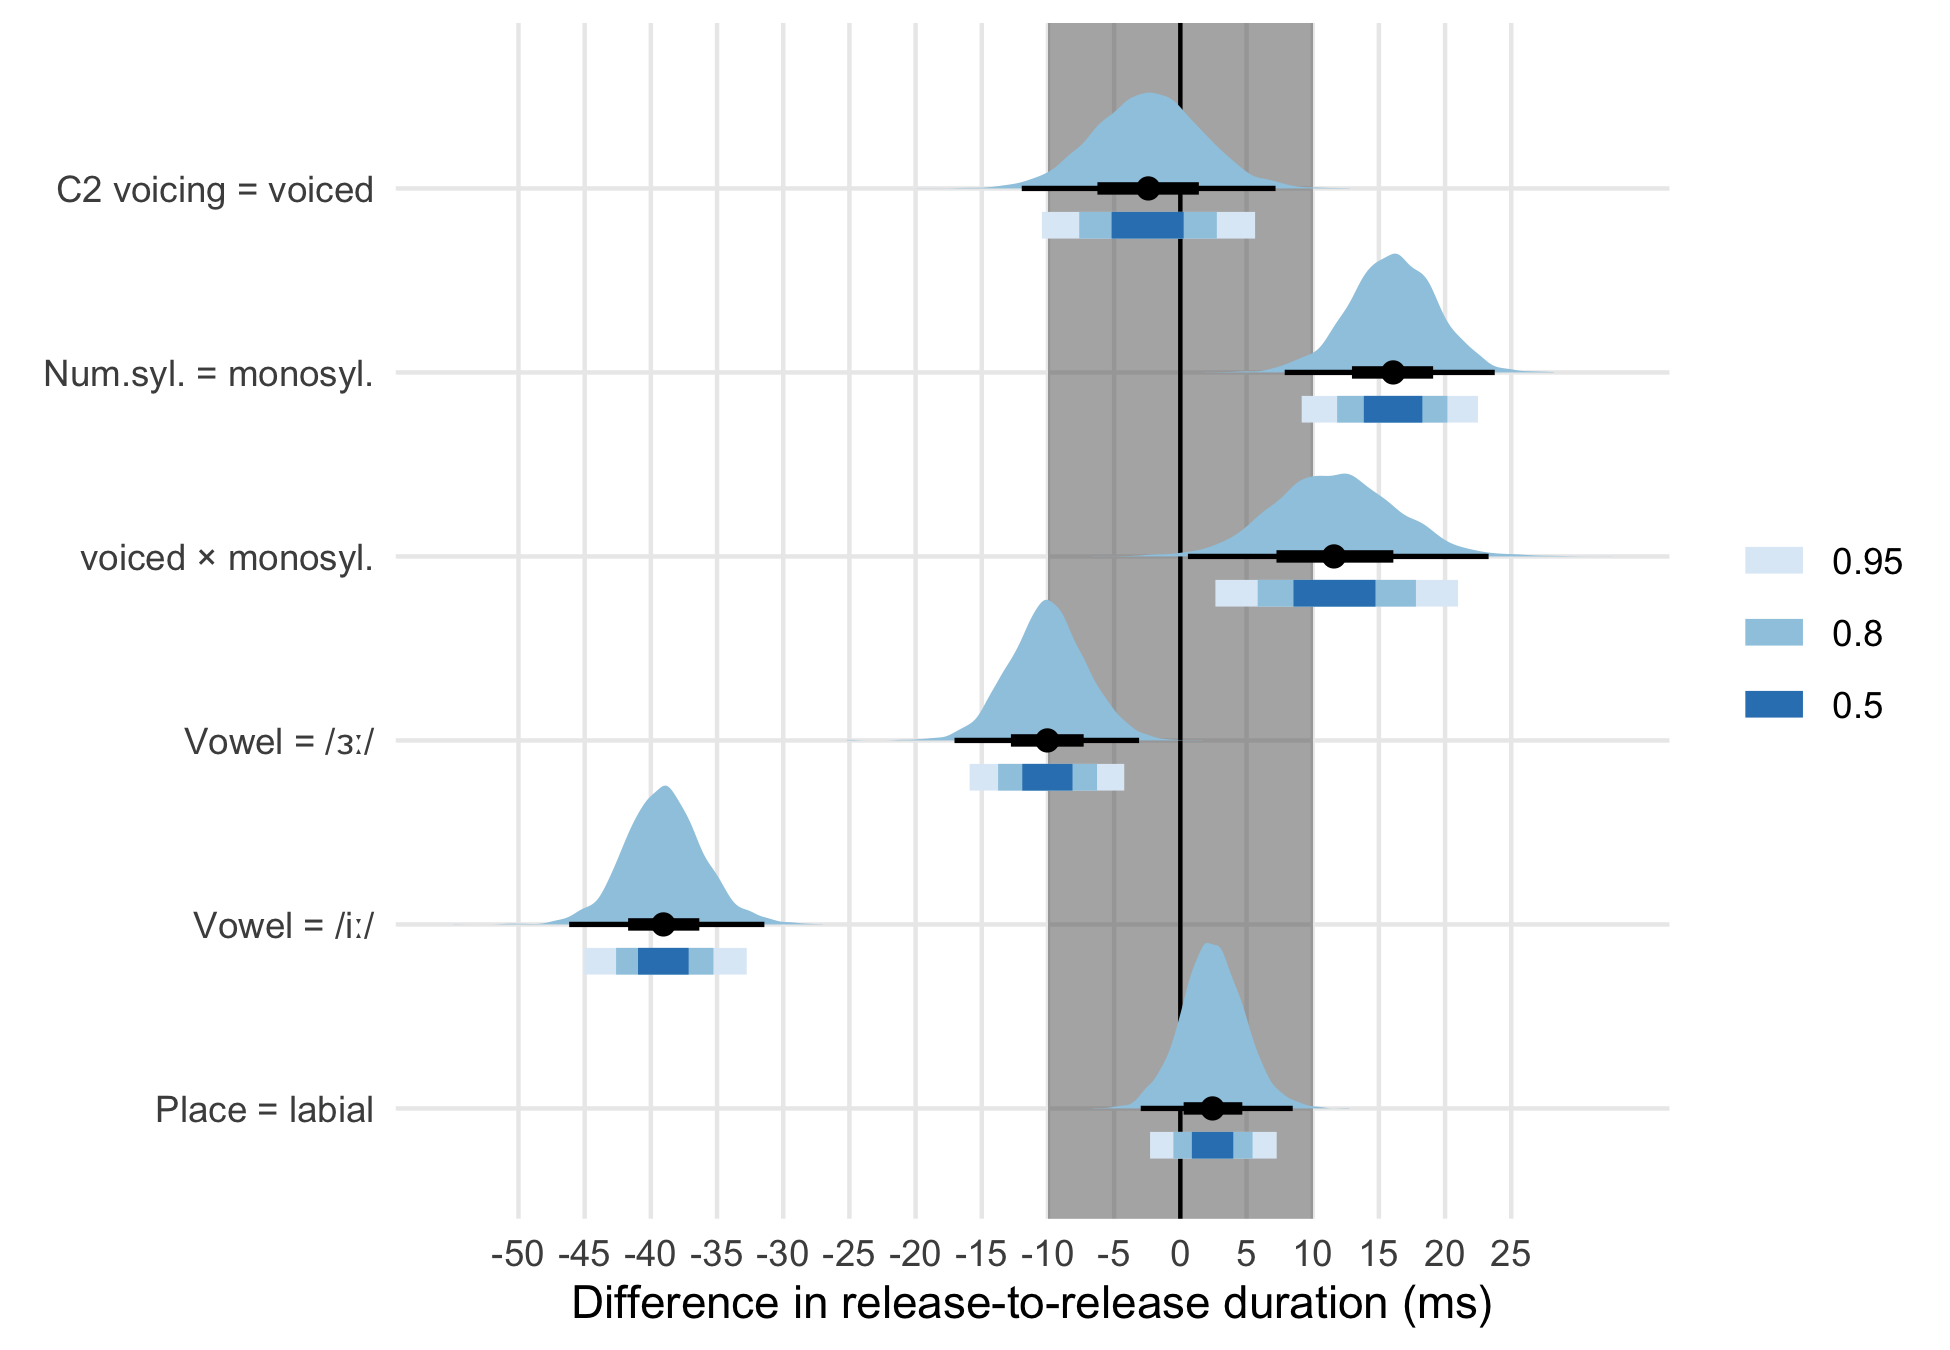
\includegraphics[width=\linewidth]{2019-english-rr_files/figure-latex/Figure1-1} \caption{Posterior distributions and Bayesian credible intervals of the effects on release-to-release duration (model 3). For each effect, the thick blue-coloured bars indicate (from darker to lighter) the 50\%, 80\%, and 95\% CI. The black point with bars are the posterior median (the point), the 98\% (thin bar) and 66\% (thicker bar) CI. The shaded grey area around 0 is the ROPE.}\label{f:Figure1}
\end{figure}

\hypertarget{vowel-duration}{%
\subsection{Vowel duration}\label{vowel-duration}}

\label{s:vow}

A Bayesian regression model was fitted to test vowel duration (model 4).
The following terms were entered: C2 voicing (voiceless, voiced), vowel
(/ɑː/, /ɜː/, /iː/), number of syllables (disyllabic, monosyllabic),
centred speech rate, all possible interactions between C2 voicing,
vowel, and number of syllables. The same random structure as in the
previous models was used (a by-speaker and by-word random intercept, and
a by-speaker random coefficient for C2 voicing).

For the prior of the intercept of vowel duration, a normal distribution
with mean 145 ms and standard deviation 30 was used
\citep{heffner1937, house1953, peterson1960, sharf1962, chen1970, klatt1973, davis1989, laeufer1992, ko2018}.
A normal distribution with mean 50 ms and standard deviation 20 was used
as the prior for the effect of voicing on vowel duration (based on the
above studies). A normal prior with mean 50 and standard deviation 25
was chosen instead for the effect of number of syllables and the
interaction C2 voicing/number of syllables. For the effects of vowel,
vowel/number of syllables interaction, and the three-way interaction
vowel/number of syllables/C2 voicing, the prior was a normal
distribution with mean 0 and standard deviation 30, based on differences
reported in the studies above. A slightly more informative prior was
used for the interaction between C2 voicing and vowel (mean = 0, SD =
20). The same priors as in the previous models were included for the
random effects.

\begin{table}

\caption{\label{tab:vow-4-table}Summary of the Bayesian regression fitted to vowel duration (model 4, see \Cref{s:vow})}
\centering
\fontsize{8}{10}\selectfont
\begin{tabular}[t]{lrrrrr}
\toprule
Predictor & Mean & SD & Q2.5 & Q97.5 & CI width\\
\midrule
Intercept & 124.91 & 5.96 & 112.94 & 136.77 & 23.83\\
Voicing = voiced & 13.65 & 5.16 & 3.73 & 24.09 & 20.36\\
Vowel = /ɜː/ & -9.03 & 5.13 & -19.08 & 1.63 & 20.71\\
Vowel = /iː/ & -36.77 & 5.00 & -46.42 & -26.67 & 19.74\\
Num. syll. = monosyllabic & 14.91 & 5.07 & 5.15 & 25.14 & 19.99\\
Speech rate (cntr.) & -18.03 & 1.48 & -20.93 & -15.29 & 5.63\\
voiced × /ɜː/ & 0.24 & 6.83 & -13.70 & 13.94 & 27.64\\
voiced × /iː/ & 6.73 & 6.59 & -6.54 & 19.26 & 25.80\\
voiced × monosyll. & 4.03 & 6.70 & -8.98 & 17.69 & 26.67\\
/ɜː/ × monosyll. & 0.53 & 7.07 & -13.57 & 14.57 & 28.15\\
/iː/ × monosyll. & -16.07 & 6.93 & -30.03 & -2.68 & 27.35\\
voiced × /ɜː/ × monosyll. & -2.94 & 9.46 & -21.37 & 15.77 & 37.14\\
voiced × /iː/ × monosyll. & 14.46 & 9.18 & -3.59 & 31.99 & 35.58\\
\bottomrule
\end{tabular}
\end{table}

\Cref{tab:vow-4-table} reports the summary of model 4, while
\Cref{f:Figure2} shows the posterior distributions and credible
intervals. The precision target was reached in the non-interacting
predictors (permitting a few milliseconds above 20), with the exeption
of the intercept. All the interactions terms have CI widths above 25 ms.
The 95\% CI of the posterior distribution of the duration of /ɑː/ is
included in the range 112.94--136.77 ms (\(\bar{\theta}\) = 124.91 ms,
SD = 5.96). The vowel /ɜː/ is 9.03 ms shorter (SD = 5.16) with CI =
{[}−19.08, 1.63{]}, while /iː/ is 36.77 ms shorter (SD = 5, 95\% CI =
{[}−46.42, −26.67{]}). C2 voicing has a small but somewhat robust
positive effect on vowel duration in disyllabic words (only partial
overlap with the ROPE without including 0). The posterior distribution
of the effect of voicing on /ɑː/ (the reference level) has mean 13.65 ms
(SD = 5.16) and 95\% CI = {[}3.73, 24.09{]}. The posterior of the
interaction of voicing with vowel when the vowel is /ɜː/ is quite spread
out around 0, with the 95\% CI between −13.70 and 13.94 ms. This
indicates that /ɑː/ and /ɜː/ are similar in their behaviour of
voicing-driven durational differences. On the other hand, the effect of
voicing is on average 6.73 ms greater (SD = 6.59, 95\% CI = {[}−6.54,
19.26{]}) when the vowel is /iː/, but the posterior overlaps with the
ROPE and it includes 0.

The magnitude of the voicing effect in disyllabic vs.~monosyllabic words
is modulated by the identity of the vowel. The posterior distribution
for the interaction C2 voicing/number of syllables when the vowel is
/ɑː/ has mean 4.03 ms (SD = 6.7) and 95\% CI {[}−8.98, 17.69{]}. This
distribution indicates the possibility for a very small increase of the
effect from disyllabic to monosyllabic words with /ɑː/, but the great
overlap with the ROPE and inclusion of 0 makes it difficult to argue for
or against a difference in effect. The three-way interaction C2
voicing/vowel/number of syllables suggests that the effect of voicing in
monosyllabic words with /ɜː/ is very similar to that of monosyllabic
/ɑː/-words (\(\bar{\theta}\) = −2.94, SD = 9.46, 95\% CI = {[}−21.37,
15.77{]}). On the other hand, the effect increases by 14.46 ms (SD =
9.18, CI = {[}−3.59, 31.99{]}) in monosyllabic words with /iː/ relative
to disyllabic /iː/-words. Note that the credible intervals of these
interaction effect are quite large, so that a wide range of values are
probable at 95\% confidence.

\begin{figure}
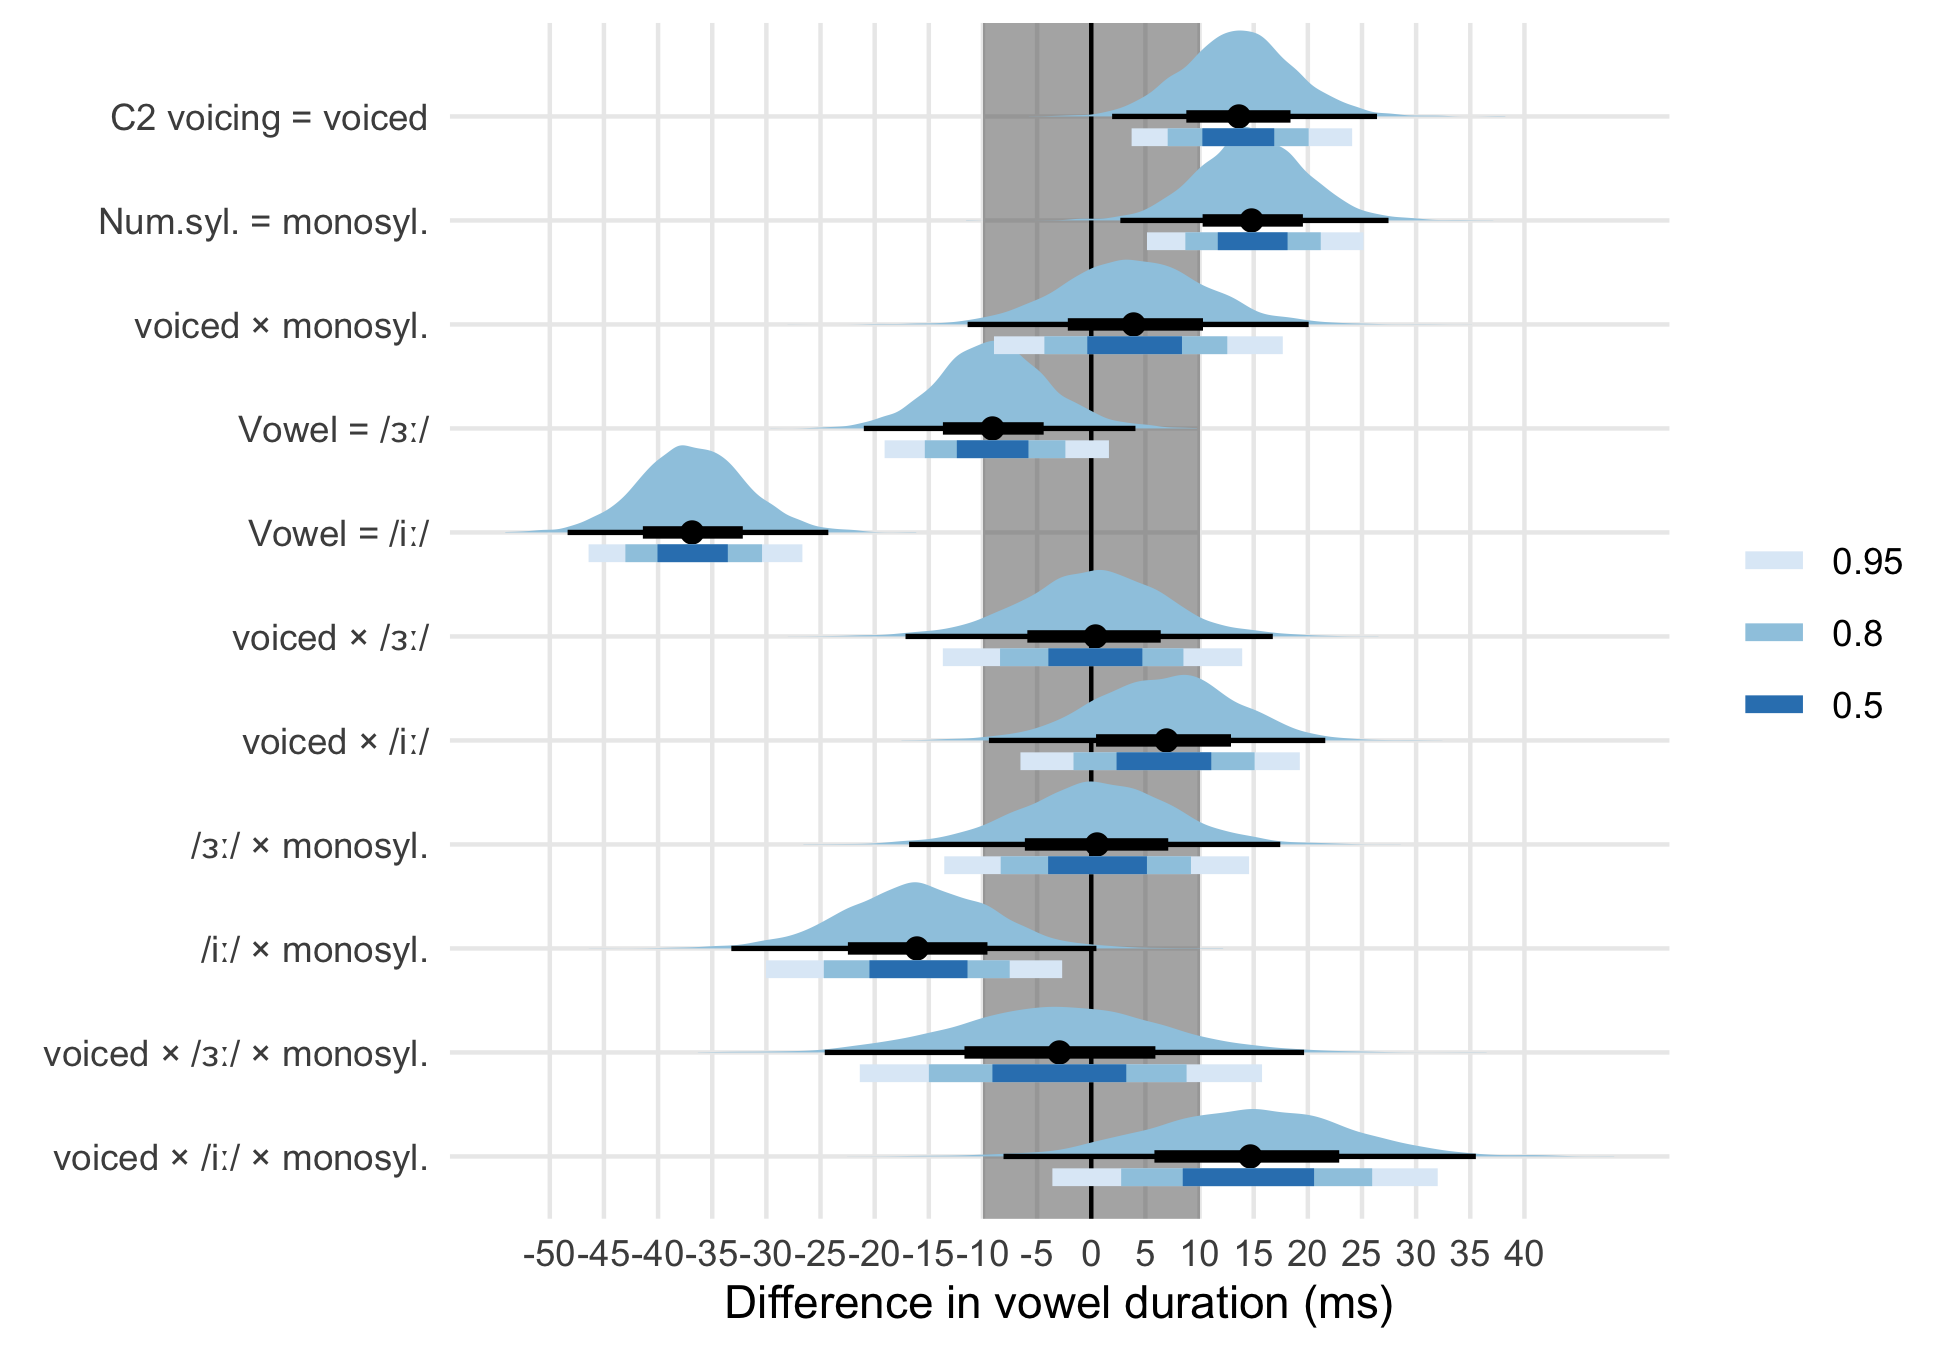
\includegraphics[width=\linewidth]{2019-english-rr_files/figure-latex/Figure2-1} \caption{Posterior distributions and Bayesian credible intervals of the effects on vowel duration (model 4). For each effect, the thick blue-coloured bars indicate (from darker to lighter) the 50\%, 80\%, and 95\% CI. The black point with bars are the posterior median (the point), the 98\% (thin bar) and 66\% (thicker bar) CI. The shaded grey area around 0 is the ROPE.}\label{f:Figure2}
\end{figure}

\hypertarget{consonant-closure-duration}{%
\subsection{Consonant closure
duration}\label{consonant-closure-duration}}

\label{s:clos}

To test various effects on C2 closure duration, model 5 was fit with
closure duration as the outcome variable and the following predictors:
C2 voicing (voiceless, voiced), C2 place of articulation (velar,
labial), number of syllables (disyllabic, monosyllabic), all
interactions between these predictor terms, and centred speech rate. The
random effects were again a by-speaker and a by-word random intercept,
and a by-speaker random coefficient for C2 voicing.

As priors, a normal distribution with mean 90 ms (SD = 20) was used for
the intercept, based on \citet{sharf1962} and \citet{luce1985}. The
means reported in these studies also indicate that the closure of the
stop in monosyllabic words is 10-30 ms shorter when the stop is voiced.
A normal distribution with mean -20 ms (SD = 10) was chosen as the prior
of the effect of C2 voicing on closure duration. The same studies
indicate that labial stops have a closure which is 10-20 ms longer than
the closure of velar stops. For the effect of C2 place, a normal
distribution with mean 15 ms (SD = 10) was used.

\begin{table}

\caption{\label{tab:clos-5-table}Summary of the Bayesian regression fitted to closure duration (model 5, see \Cref{s:clos})}
\centering
\fontsize{8}{10}\selectfont
\begin{tabular}[t]{lrrrrr}
\toprule
Predictor & Mean & SD & Q2.5 & Q97.5 & CI width\\
\midrule
Intercept & 74.75 & 2.86 & 69.07 & 80.59 & 11.52\\
Voicing = voiced & -20.79 & 3.06 & -26.77 & -14.74 & 12.03\\
C2 place = labial & 5.19 & 2.77 & -0.03 & 10.76 & 10.79\\
Num. syll. = monosyllabic & 2.98 & 2.90 & -2.80 & 8.77 & 11.58\\
Speech rate (cntr.) & -9.21 & 1.26 & -11.71 & -6.74 & 4.97\\
voiced × labial & 1.37 & 3.94 & -6.79 & 8.93 & 15.72\\
voiced × monosyll. & 1.82 & 4.06 & -6.08 & 9.70 & 15.78\\
labial × monosyll. & -0.74 & 4.02 & -8.95 & 6.88 & 15.83\\
voiced × labial × monosyll. & 6.41 & 5.66 & -4.72 & 17.45 & 22.17\\
\bottomrule
\end{tabular}
\end{table}

The summary of model 5 is shown in \Cref{tab:clos-5-table}. See
\Cref{f:Figure3} for the posteriors and credible intervals of the
effects. The 96\% CI width of all the terms, with the exception of the
three-way interaction (voicing/place/number of syllables), is below 20
ms (the precision goal has been reached). The posterior distribution of
the intercept for closure duration (corresponding to the duration of
voiceless velar stops in disyllabic words) has mean 74.75 ms (SD = 2.86)
and 95\% CI = {[}69.07, 80.59{]}. The effect of C2 voicing on closure
duration is robustly negative, between −26.77 and −14.74 ms (95\% CI).
The posterior mean of this effect is −20.79 ms (SD = 3.06). A very small
positive effect of place of articulation (labial) is suggested by the
95\% CI from −0.03 to 10.76 ms (\(\bar{\theta}\) = 5.19 ms, SD = 2.77).
A possibly even smaller effect of number of syllables or no effect at
all can be inferred from the posterior distribution which has mean 2.98
ms and SD 2.9 (95\% CI = {[}−2.8, 8.77{]}). Note that the 95\% CIs of
the posterior distributions of all the effects, with the exception for
the effect of voicing, are within the ROPE around 0, meaning that they
can be interpreted as practically null effects.

\begin{figure}
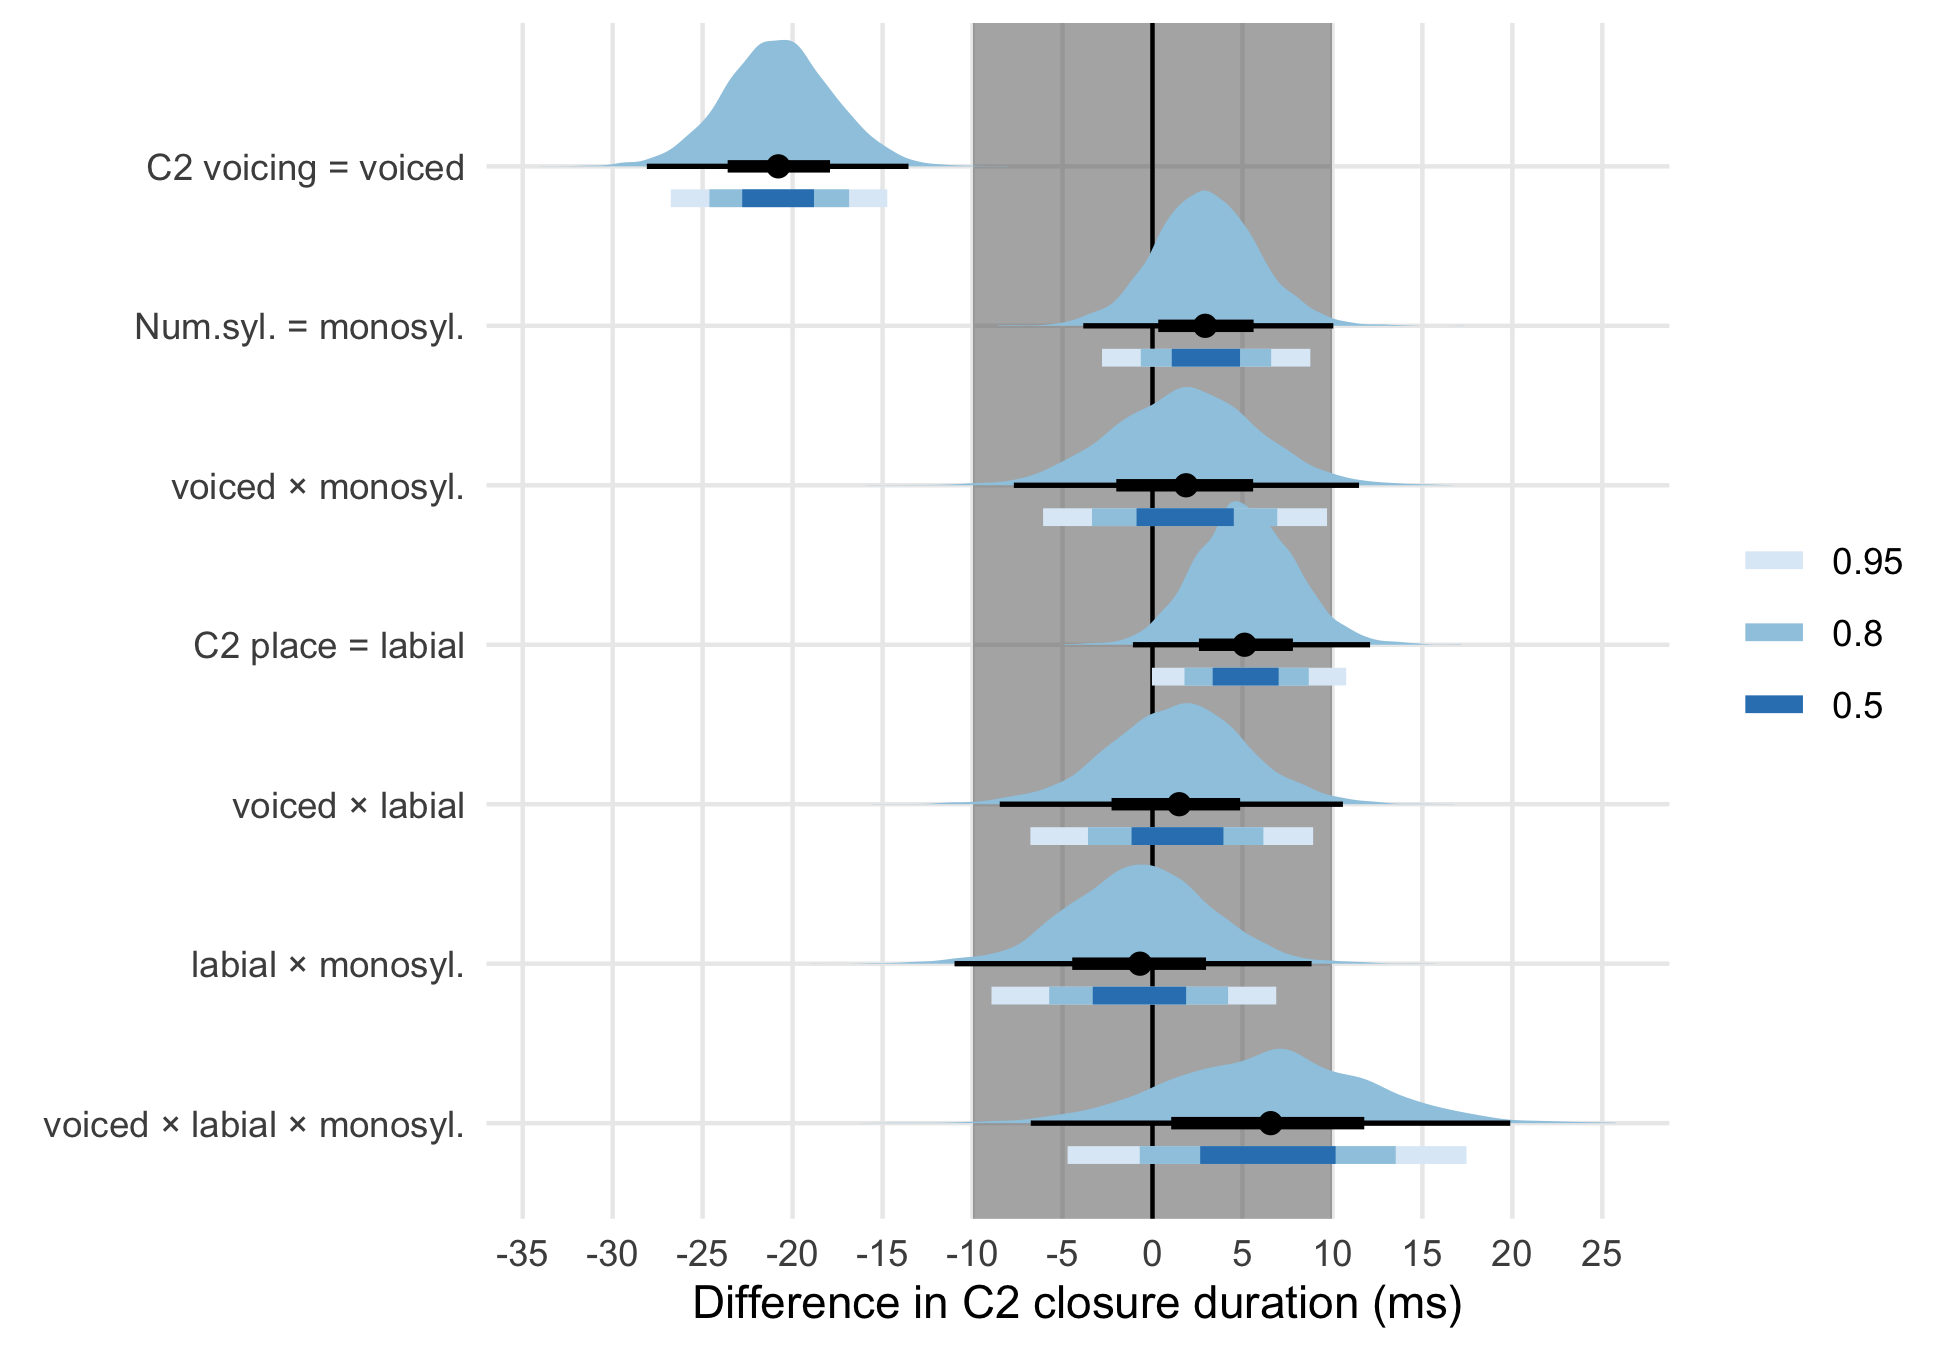
\includegraphics[width=\linewidth]{2019-english-rr_files/figure-latex/Figure3-1} \caption{Posterior distributions and Bayesian credible intervals of the effects on closure duration (model 4). For each effect, the thick blue-coloured bars indicate (from darker to lighter) the 50\%, 80\%, and 95\% CI. The black point with bars are the posterior median (the point), the 98\% (thin bar) and 66\% (thicker bar) CI. The shaded grey area around 0 is the ROPE.}\label{f:Figure3}
\end{figure}

\hypertarget{discussion}{%
\section{Discussion}\label{discussion}}

This study set out to build on the results discussed in
\citet{coretta2019k} by investigating durational properties of the
release-to-release interval in English monosyllabic and disyllabic
words. It was expected that the release-to-release interval would not be
affected by C2 voicing in disyllabic words but it would in monosyllabic
words. Moreover, a conceptual replication of studies on the effect of
consonant voicing on vowel and closure durations was sought, with a
focus on comparing the effect in mono- vs.~disyllabic words. This
section discusses in turn the results in relation to the
release-to-release interval duration (\Cref{s:rr-disc}) and to vowel and
closure durations (\Cref{s:vc-disc}) by comparing them with the
hypotheses of this study. \Cref{s:gen-disc} synthesises and links these
findings back to the articulatory grounding of the temporal properties
of the release-to-release interval in mono- and disyllabic words
(\Cref{s:intro}). Limitations and future work are also discussed.

\hypertarget{release-to-release-interval}{%
\subsection{Release-to-release
interval}\label{release-to-release-interval}}

\label{s:rr-disc}

The first question (see \Cref{s:hypo}) asked whether the voicing of C2
in disyllabic and monosyllabic words in English influences the duration
of the release-to-release interval. \citet{coretta2019k} showed that the
release-to-release interval duration is not affected by C2 voicing in
disyllabic words of Italian and Polish. The hypotheses were that, in
English, the interval is not affected in disyllabic words, like in
Italian and Polish, but that it is in monosyllabic words. In sum, the
results of this study indicate that the release-to-release duration of
disyllabic words in English is relatively stable independent of whether
C2 is voiceless (like in /tɑːpəs/) or voiced C2 (/tɑːbəs/). On the other
hand, the release-to-release in monosyllabic words is longer if C2 is
voiced (like in /tɑːb/ vs.~/tɑːp/).

Two pre-registered Bayesian regression models were fitted to the
release-to-release duration (model 1-2). The established ROPE target has
not been achieved (see \Cref{s:sample-size}). An exploratory model
(model 3) including all predictors from model 1 and 2 resulted in higher
estimate precision (CI widths below 20 ms). The results of model 3
suggest a negligible effect of C2 voicing on the interval duration in
disyllabic words (hypothesis 1a), with a 95\% probability that the true
effect is between −10 and +5 ms. At lower levels of probability, the
posterior distribution indicates an effect between −6 and 1 ms (60\%
probability). If the voicing of C2 is conditioning the duration of the
release-to-release interval, this effect is very small.

The possible small effect of C2 voicing in disyllabic words could be
related to an annotation bias which affects the identification of stop
releases. English voiceless stops are generally followed by aspiration,
and the glottal friction that makes up aspiration could mask the burst
of the release. If the release of the post-vocalic voiceless stops is
annotated later than the actual release (by mistaking peaks in the
aspiration noise for the release burst), this could lead to longer
release-to-release durations when C2 is voiceless compared to when it is
voiced. Such annotation bias could explain the quite small negative
effect of voicing on the interval duration, and why it is in the
opposite direction of the one predicted for monosyllabic words
(i.e.~\emph{longer} release-to-release when C2 is voiced).

On the other hand, the release-to-release interval in monosyllabic words
is longer when C2 is voiced (for example, /tɑːb/) vs.~when it is
voiceless (/tɑːp/). The interaction term between number of syllables in
the word and C2 voicing is positive, between +2.5 and +21 ms (at 95\%
probability), which means that the effect of C2 voicing increases by 2.5
to 21 ms in monosyllabic words relative to the effect in disyllabic
words. This result is compatible with hypothesis 1b that the
release-to-release interval is longer in monosyllabic words with a
voiced C2 than in monosyllabic words with a voiceless C2. As discussed
in \Cref{s:intro}, the absence of release-to-release isochrony in
monosyllabic words is possibly due to the absence of a second vowel
which would constitute the left articulatory anchor for vowel isochrony,
which in turn is argued to be the necessary element for the
release-to-release temporal stability (also see \Cref{s:gen-disc}).

The second question posed at the beginning of the paper was about other
effects on the release-to-release duration. As expected by hypothesis
2a, the release-to-release is longer in monosyllabic than in disyllabic
words. At 95\% probability, the effect of number of syllables (from di-
to monosyllabic) is between 9 and 22.5 ms. As for hypothesis 2b, the
results are more robust for /iː/ than for /ɜː/. When the vowel is /iː/,
the release-to-release interval is 33 to 45 ms shorter compared with an
interval with /ɑː/. The posterior distribution of the effect when the
vowel is /ɜː/ substantially overlaps with the ROPE, although it tends
towards the negative side. If there is an effect with this vowel
compared to /ɑː/, it is negative and possibly around −10 ms. Finally,
hypothesis 2c is not unequivocally corroborated. The posterior
distribution of the effect of C2 place of articulation (labial) has very
high precision (9.5 ms) and it is between 0 and 5 ms (at somewhat less
than 80\% probability). However, it lies within the ROPE and it is very
close to 0.

\hypertarget{vowel-and-closure-duration}{%
\subsection{Vowel and closure
duration}\label{vowel-and-closure-duration}}

\label{s:vc-disc}

Question 3 addressed the effect of voicing on vowel and closure
duration, and the possible differences between disyllabic and
monosyllabic words. The results do indicate an effect of voicing on
vowel duration (as expected based on previous work on English), but the
effect found in this study was estimated to lie between 4 and 25 ms.
This range of values is very similar to that reported in
\citet{coretta2019k} for Italian and Polish disyllabic words (the 95\%
confidence interval for the effect in these languages is {[}8, 25{]}),
monosyllabic words were not tested). When compared to the values in
previous studies that investigated disyllabic words
\citep{sharf1962, klatt1973, davis1989}, the effect size found in this
study tends towards smaller values. However, note that the posterior
distribution of the effect in the current study is entirely contained in
the meta-analytical posterior distribution of the effect in the other
studies, which roughly ranges between −15 and +65 ms (see Supplement A).
Thus, we can assume that the deviation of this study from previous ones
is not substantial. As for the effect of number of syllables on vowel
duration, a similar effect to that of voicing was found, whereby vowel
durations increase by 5 to 25 ms in monosyllabic words compared to
disyllabic words. This relation corresponds to what has previously been
reported in the literature. Finally, given that the 95\% CIs of the
effects of voicing and number of syllables overlap with the right side
of the ROPE without including 0, the data supports positive effects, but
inference on their magnitude should be carefully weighted.

It was expected that the voicing effect on vowels would be stronger in
monosyllabic than in disyllabic words (hypothesis 3). The credible
intervals of the posterior distributions from model 4, which are larger
than the ROPE, make interpretation less straightforward. At 80\%
probability, the difference in voicing effect between mono- and
disyllabic words is between −5 and +12.5 ms. The distribution is skewed
towards the positive side, and this is compatible with results from
previous studies, although the CI includes 0. The magnitude, however, is
considerably lower than what previously reported. However, more data is
needed to reach a sensible estimate precision and increase inferential
certainty.

The three-way interaction between C2 voicing, vowel, and number of
syllables reveals that the effect in monosyllabic words with the vowel
/ɜː/ is similar to that with /ɑː/. On the other hand, the effect is
larger if the vowel is /iː/. Model 4 estimates an effect increase of
about 14.5 ms ({[}−4.27, 33.41{]}). Note that the credible interval is
very wide (38 ms) and it spans over both negative and positive values,
although tends more towards the latter. Moreover, the vowel /iː/
followed by a voiceless stop has, according to the model, the same
duration in monosyllabic and disyllabic words. While it is not clear why
the vowel should have the same duration in these contexts, this pattern
suggest a possible process of /iː/ shortening in monosyllabic words.
More research is warranted in relation to the observed patterns.

Turning now to consonants, it was expected for voiced closures to be
longer than voiceless closures, but there was no specific hypothesis
concerning the effect of number of syllables on the effect of voicing on
closure durations. C2 voicing has a robust negative effect on closure
duration, so that voiced closures are 14.6-26.8 ms shorter than
voiceless closures. The effects of number of syllables, place, and
interactions all have credible intervals that are narrower than 20 ms
(the ROPE width) but they lie entirely within the ROPE around 0. If
these variables do have an effect on closure duration, the present
analysis suggests that the means of these effects are between 0 and 5
ms. These values are smaller than those reported in \citet{sharf1962},
which instead indicated a difference of 15 ms between velar and labial
closure durations.

As a general trend, although an effect of C2 voicing on vowel and
closure duration was found, the voicing-driven differences in vowel and
closure duration found here are smaller than those known from the
literature, and considerably so in the case of vowels. A possible reason
for this discrepancy could be found in problems arising from Type M
errors (as briefly discussed in \Cref{s:intro}), and in differences of
speech rate, as evidenced by comparing average segment durations. While
the model's intercept of vowel duration in this study is approximately
125 ms (SD = 5.89), the mean vowel duration in the studies surveyed in
the meta-analysis (Supplement A) is 150 ms (SD = 36). These longer
durations may indicate lower speech rates in older studies and so the
effect of voicing may have been greater there than at higher speech
rates, assuming a linear increase of the effect. However, the ratio
between vowel duration and the effect of voicing differs (vowels
increase by a third of their total duration in this study vs.~half in
previous work). Ko's findings \citeyear{ko2018} support the idea that
the voicing effect (and the vowel-to-consonant ratio) are not stable
across speaking rates, with the consequence that differences are
enhanced at decreased speaking rates. More studies like \citet{ko2018}
are needed to settle the issue of the diverging results.

\hypertarget{general-discussion}{%
\subsection{General discussion}\label{general-discussion}}

\label{s:gen-disc}

\citet{coretta2019k} proposes that the voicing-related adjustments in
the relative timing of the closure onset within an isochronous speech
interval (acoustically identified as the release-to-release interval) is
the diachronic precursor of the cross-linguistically widespread effect
of voicing on vowel
duration.\footnote{Note that isochrony here is intended as pertaining the context of voiceless vs. voices stops only.}
Given that the duration of the release-to-release interval in Italian,
Polish, and English disyllabic words is arguably not affected by the
voicing of the post-vocalic consonant, the relative durations of vowel
and closure are thought to depend on the timing of the VC boundary
within that interval. A later VC boundary in the context of voiced stops
implies a longer vowel and a shorter closure relative to the voiceless
context, while, vice versa, an earlier boundary in the context of
voiceless stops produces a shorter vowel and a longer closure relative
that voiced context. Behind the differential timing of the VC boundary
within the release-to-release interval, several other accounts can be
envisaged, like accounts relating to laryngeal and supraglottal
adjustments \citep{halle1967, begus2017, coretta2019c}.

As discussed in \Cref{s:gest}, a prerequisite of the articulatory
account proposed here for the emergence of the voicing effect is the
temporal stability of the acoustic release-to-release interval and of
the related articulatory gestures. However, it was expected that English
mono-syllabic words do not show such temporal stability, even though the
voicing effect is present in this context and allegedly even grater than
in disyllabic words (on the latter point, cf.~with Supplement A and this
study, where a less clear picture emerged).

As mentioned at the end of \Cref{s:gest}, the absence of temporal
stability and presence of the voicing effect in monosyllabic words can
be reconciled by drawing from known mechanisms of perceptual
enhancement. Perceptual biases, like the ones proposed by perceptual
accounts of the voicing effect
\citep{javkin1976, kluender1988, sanker2019}, can contribute to the
increase of the effect of voicing, for example as a means to enhance the
perceptual difference of voiceless vs.~voiced stops
\citep{lisker1974, lisker1986, stevens1989}. In particular, vowels can
be further lengthened when followed by voiced stops and/or further
shortened when followed by voiceless stops, so as to produce a greater
and more perceptible difference.

In the case of disyllabic words, movements of the VC boundary within the
isochronous interval will logically affect both vowel duration and
closure duration, while the release-to-release would not be affected and
vowel-to-vowel isochrony would be preserved. On the other hand, the
absence of a second vowel acting as temporal articulatory anchor (as per
vowel-to-vowel isochrony) in monosyllabic words would allow articulatory
stretching or compression to operate independently on the vocalic and
the consonantal gestures. In the monosyllabic context, the gestural
duration of vowels and following consonants can be modified in such a
way that could result in a change in timing of the onset of the
consonant closing gesture and in the disruption of the
release-to-release isochrony.

The presence of a voicing effect with absence of release-to-release
temporal stability could be obtained, for example, by keeping the
vocalic gesture when the following stop is voiced active for a longer
time relative to when the following stop is voiceless. Although more
research is needed in this area, the articulatory studies in
\citet{raphael1972} and \citet{de-jong1991} do suggest that the vocalic
gesture in monosyllabic words is executed for a prolonged time when the
following consonant is voiced. While differences in magnitude of the
voicing effect should be replicated in future studies, the potentially
greater effect of voicing in monosyllabic words could be ascribed to the
fact that, while vowel-to-vowel isochrony constraints how vowels and
consonants can be produced in disyllabic words, mechanisms affecting the
VC boundary (articulatory and/or perceptual) in monosyllabic words are
less constrained due to the non-application of vowel-to-vowel isochrony.

\hypertarget{conclusion}{%
\section{Conclusion}\label{conclusion}}

This paper set out to investigate temporal properties of the so-called
`voicing effect', by which vowels are shorter when followed by voiceless
stops and longer when followed by voiced stops. \citet{coretta2019k}
proposes that the voicing effect emerges via a mechanism of relative
timing of the VC boundary within a temporally stable interval. Such
interval was argued to be the interval between two consecutive releases,
as evidenced by acoustic data from Italian and Polish disyllabic words.
The temporal stability of the release-to-release in relation to
consonantal voicing is thought to derive from two properties of gestural
phasing, namely the isochrony of the distance between the vowels in a
VCV sequence, and in-phase alignment of onset consonants and the
following vowel. On the other hand, the lack of an articulatory anchor
(a second vowel) in monosyllabic words would allow the
release-to-release duration to be affected by C2 voicing and differ in
the monosyllabic context.

This study adds to the current status of knowledge on temporal aspects
of the voicing effect by showing that the release-to-release interval is
not affected by C2 voicing in English disyllabic words, as in Italian
and Polish, and that, instead, it is longer in monosyllabic words when
C2 is voiced. While the timing of the VC boundary within the
release-to-release in disyllabic words affects both vowel and closure
durations in a logically dependent way, vowel and closure durations can
be modulated more independently in monosyllabic words. The less
constrained operation of production/perceptual mechanisms affecting the
timing of the VC boundary was argued to be the reason for the seemingly
greater effect of voicing reported for monosyllabic words. The data in
this study, and the cumulative evidence from previous studies as evinced
by a Bayesian meta-analysis, however, do not equivocally provide support
for a difference in the effect between mono- and disyllabic words, and
future work is necessary to shed light on the matter.

To conclude, the results of this study suggest some directions of
research. Future studies should further investigate the articulatory
temporal patterns of vocalic and consonantal gestures in disyllabic
words. In particular, a complete assessment of the isochrony (or lack
thereof) of consecutive vocalic gestures should include a variety of
oppositions, involving voicing, place of articulation, number of
consonants, syllabic affiliation, and prosodic contexts. Moreover, work
is needed to shed light on the timing of the consonant closing gesture
relative to the articulatory gesture of the preceding vowel in voiceless
vs.~voiced stops. Finally, the scenario of emergence of the voicing
effect offered here should be examined in in relation to other
consonantal effects on vowel duration, like other laryngeal effects and
effects of manner of articulation.

\bibliography{linguistics}

\end{document}
